\chapter*{Appendix}
\addcontentsline{toc}{chapter}{Appendix}
\scriptsize
\section{Intermediate results for parameter optimisation}
\subsection{IB4010}
\begin{figure}[hb!]
\centering
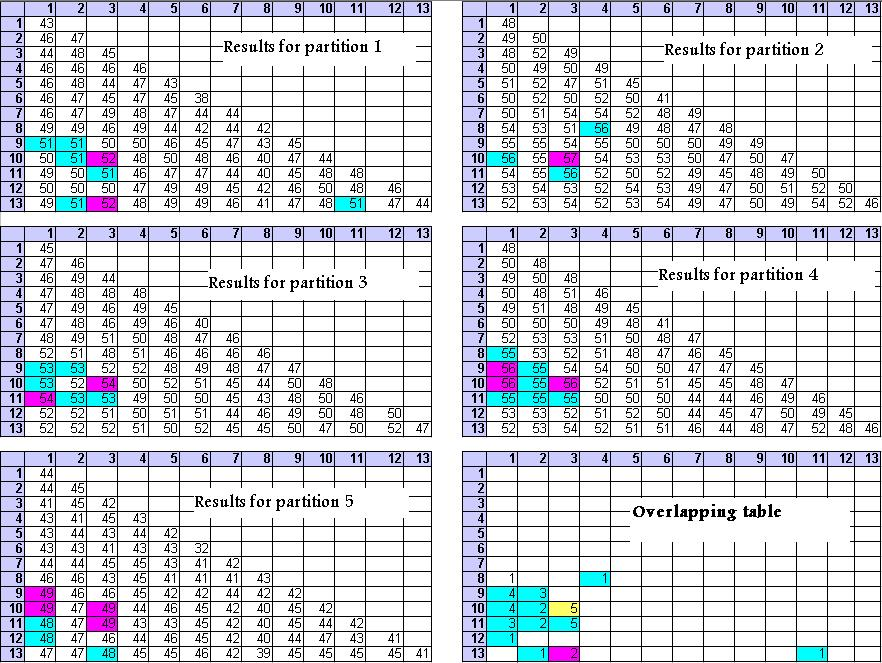
\includegraphics[scale = 0.85]{IB4010_optimisation.jpg}
\caption{Using 5-fold Cross-Validation for parameter optimisation for IB4010}
\label{Using 5-fold Cross-Validation for parameter optimisation for IB4010}
\end{figure}

\pagebreak

\subsection{IS1008c}
\begin{figure}[hb!]
\centering
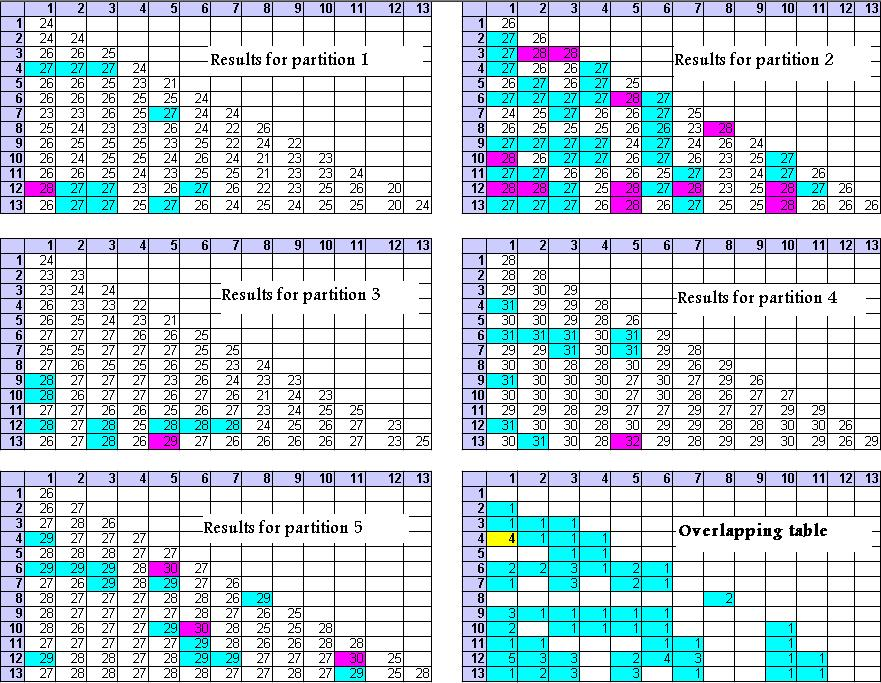
\includegraphics[scale = 0.85]{IS1008c_optimisation.jpg}
\caption{Using 5-fold Cross-Validation for parameter optimisation for IS1008c}
\label{Using 5-fold Cross-Validation for parameter optimisation for IS1008c}
\end{figure}

%What goes in the appendices? Any material which impedes the smooth development of your
%presentation, but which is important to justify the results of a thesis. Generally it is material
%that is of too nitty-gritty a level of detail for inclusion in the main body of the thesis, but which
%should be available for perusal by the examiners to convince them sufficiently. Examples include
%program listings, immense tables of data, lengthy mathematical proofs or derivations, etc.

%\section{Source code in Java}
%\subsection{Calculating passage score}
%
%\lstset{numbers=left, stepnumber=1,breaklines=true}%,basicstyle=\footnotesize ,numberstyle=\footnotesize , showspaces=false, showstringspaces=false, showtabs=false, breakatwhitespace=true }
%
%\lstset{language=Java, caption=Calculating Passage Score, label=DescriptiveLabel}
%\lstset{frame=shadowbox, rulesepcolor=\color{blue}}
%%\begin{frame}
%\lstinputlisting{code.java}
%%\end{frame}
%
%
%\section{Source code of the procedure Determining True Statement}
%%\begin{framed}
%%\begin{lstlisting}…\end{lstlisting}
%%or \lstinputlisting{…}
%%\end{framed}


\section{List of stopwords}
\small 
\textit{i, a, about, above, an, are, as, at, am, and, be, been, being, but, by, do, does, done, did, for, he, her, hers, herself, his, him, himself, how, in, is, it, its, itself, me, my, mine, myself, nor, of, on, or, our, ours, ourself, ourselves, so, she, that, the, they, them, their, theirs, these, themself, themselves, this, those, to, uh, um, up, us, really, very, was, were, we, well, will, with, what, when, where, which, who, whom, whose, why, yet, you, your, yours, yourself, yourselves.
}
\normalsize